\subsection{Numerical Experiments}
In the following we present a series of experiments on test cases in order to verify the properties of the methods presented above. All experiments are performed using Montecarlo simulations to approximate the mean exit time and the exit probability. For each realization (or trajectory) of the Brownian motion we compute $\tau$ and $\phi$ using DEM or CEM. We denote by $M$ the number of simulated trajectories and approximate the quantities of interest as
\begin{equation}\label{eq:MonteCarlo}
\begin{aligned}
	\E(\tau_h^d) &\approx \frac{1}{M} \sum_{j=1}^M (\tau_h^d)_j, \\
	\E(\tau_h^c) &\approx \frac{1}{M} \sum_{j=1}^M (\tau_h^c)_j, \\
	\E(\phi_h^d) &\approx \frac{1}{M} \sum_{j=1}^M (\phi_h^d)_j, \\	
	\E(\phi_h^c) &\approx \frac{1}{M} \sum_{j=1}^M (\phi_h^c)_j, \\	
\end{aligned}
\end{equation}
where $(\tau_h^d)_j, (\phi_h^d)_j$ denote the values of $\tau$ and $\phi$ given by the $j$-th trajectory of DEM (respectively CEM). 
\subsubsection{One-Dimensional Case}
We consider problem \eqref{eq:GeneralModel} in case $d = 1$. Given $f,g$ defined on an interval $D = \left[l,r\right]$ and a Brownian motion $W(t)$, let us consider the following one dimensional SDE
\begin{equation}\label{eq:OneDModel}
\left \{
\begin{aligned}
	dX(t) &= f(X(t)) dt + g(X(t))dW(t), && 0 < t \leq T, \\
	X(0)  &= X_0, && X_0 \in D.
\end{aligned} \right .
\end{equation}
In this case, the boundary of $D$ consists of the two points $\{l,r\}$. In order for the problem of the determination of $\tau$ to be meaningful, at least one of the two points should be endowed with a killing boundary condition. 

\vspace{2mm}
\noindent \textbf{Estimation of the exit time.} We consider as a domain for \eqref{eq:OneDModel} the interval $D = \left[-1,1\right]$, final time $T = 5$ and the following functions
\begin{align}\label{eq:FunctionsOneDSmooth}
\begin{split}
	f(x) &= -V'(x), \text{ where } V(x) = 0.1(8x^4 - 8x^2 + x + 2), \\
	g(x) &= \sigma = 3.
\end{split}
\end{align}
We approximate the value of $\tau$ with a Montecarlo simulation of $\tau_h^d$ and $\tau_h^c$ computed as in \eqref{eq:TauDEM} and \eqref{eq:TauCEM} from the solutions provided by DEM and CEM respectively. In order to verify the order of convergence of the methods, we let $N$ vary in the set $2^i,i=3,\dots,12$ and we fix the number of trajectories $M$ to $10^4$. In this way, the error caused by the Montecarlo estimation should not spoil the order of convergence. We compute the error with respect to the analytic value of the mean exit time in this simple case (see Appendix \ref{sec:Appendix1}). In Figure \ref{fig:OrdersOneD} we show the errors obtained fixing $X_0 = 0$ in both the cases of killing and reflecting boundary conditions in $x = 1$. Moreover, in Figure \ref{fig:ApproxOneD} we show an approximation of $\tau$ obtained with the two methods with $h = T/128$ and $M = 10^3$ for a set of 10 initial values equispaced along $D$. It is possible to remark that computing the probability of exit between two consecutive timesteps as in \eqref{eq:CEMProbHalfSpace} allows correcting the overestimation of $\tau$ obtained simply using DEM. As far as the performances are concerned, we remark that the computational time required by CEM is higher than for DEM if the same value of $h$ is employed. On the other hand, fixing the error, CEM is faster than DEM in this case.

\begin{figure}[t]
    \centering
    \begin{subfigure}{0.49\linewidth}
        \centering
        \resizebox{1\linewidth}{!}{% This file was created by matlab2tikz.
%
%The latest updates can be retrieved from
%  http://www.mathworks.com/matlabcentral/fileexchange/22022-matlab2tikz-matlab2tikz
%where you can also make suggestions and rate matlab2tikz.
%
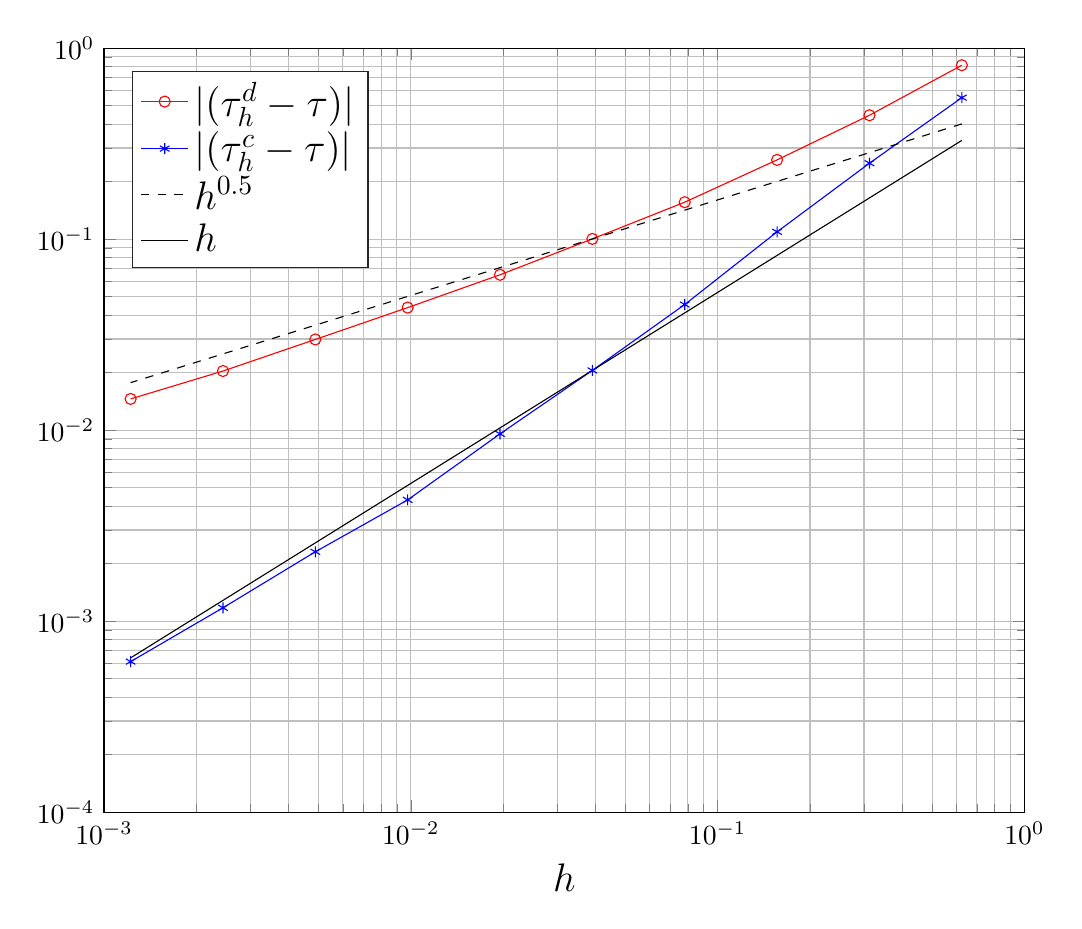
\begin{tikzpicture}

\begin{axis}[%
width=4.602in,
height=3.82in,
at={(0.772in,0.516in)},
scale only axis,
xmode=log,
xmin=0.001,
xmax=1,
xminorticks=true,
xlabel={$h$},
xlabel style = {font=\Large},
xmajorgrids,
xminorgrids,
ymode=log,
ymin=0.0001,
ymax=1,
yminorticks=true,
ymajorgrids,
yminorgrids,
axis background/.style={fill=white},
legend style={at={(0.03,0.97)},anchor=north west,legend cell align=left,align=left,draw=white!15!black,font=\Large}
]
\addplot [color=red,solid,mark=o,mark options={solid}]
  table[row sep=crcr]{%
0.625	0.814121166527388\\
0.3125	0.445308666527388\\
0.15625	0.260074291527388\\
0.078125	0.156160229027388\\
0.0390625	0.100300854027388\\
0.01953125	0.0650840571523877\\
0.009765625	0.0438213618398876\\
0.0048828125	0.0298496821523877\\
0.00244140625	0.0203989985586377\\
0.001220703125	0.0145757563711377\\
};
\addlegendentry{$|\E(\tau_h^d - \tau)|$};

\addplot [color=blue,solid,mark=asterisk,mark options={solid}]
  table[row sep=crcr]{%
0.625	0.550496166527388\\
0.3125	0.249839916527388\\
0.15625	0.109277416527388\\
0.078125	0.0454727290273877\\
0.0390625	0.0205547602773877\\
0.01953125	0.00956257277738766\\
0.009765625	0.00431550246488765\\
0.0048828125	0.00230768996488766\\
0.00244140625	0.00117487746488766\\
0.001220703125	0.000614086449262655\\
};
\addlegendentry{$|\E(\tau_h^c - \tau)|$};

\addplot [color=black,dashed]
  table[row sep=crcr]{%
0.625	0.401203416109551\\
0.3125	0.283693656166271\\
0.15625	0.200601708054775\\
0.078125	0.141846828083136\\
0.0390625	0.100300854027388\\
0.01953125	0.0709234140415679\\
0.009765625	0.0501504270136938\\
0.0048828125	0.0354617070207839\\
0.00244140625	0.0250752135068469\\
0.001220703125	0.017730853510392\\
};
\addlegendentry{$h^{0.5}$};

\addplot [color=black,solid]
  table[row sep=crcr]{%
0.625	0.328876164438203\\
0.3125	0.164438082219101\\
0.15625	0.0822190411095506\\
0.078125	0.0411095205547753\\
0.0390625	0.0205547602773877\\
0.01953125	0.0102773801386938\\
0.009765625	0.00513869006934691\\
0.0048828125	0.00256934503467346\\
0.00244140625	0.00128467251733673\\
0.001220703125	0.000642336258668364\\
};
\addlegendentry{$h$};

\end{axis}
\end{tikzpicture}%
 }  
        \caption{Killing boundary in $x = 1$}
        \label{fig:KillOneD}
    \end{subfigure}
    \begin{subfigure}{0.49\linewidth}
        \centering
        \resizebox{1\linewidth}{!}{% This file was created by matlab2tikz.
%
%The latest updates can be retrieved from
%  http://www.mathworks.com/matlabcentral/fileexchange/22022-matlab2tikz-matlab2tikz
%where you can also make suggestions and rate matlab2tikz.
%
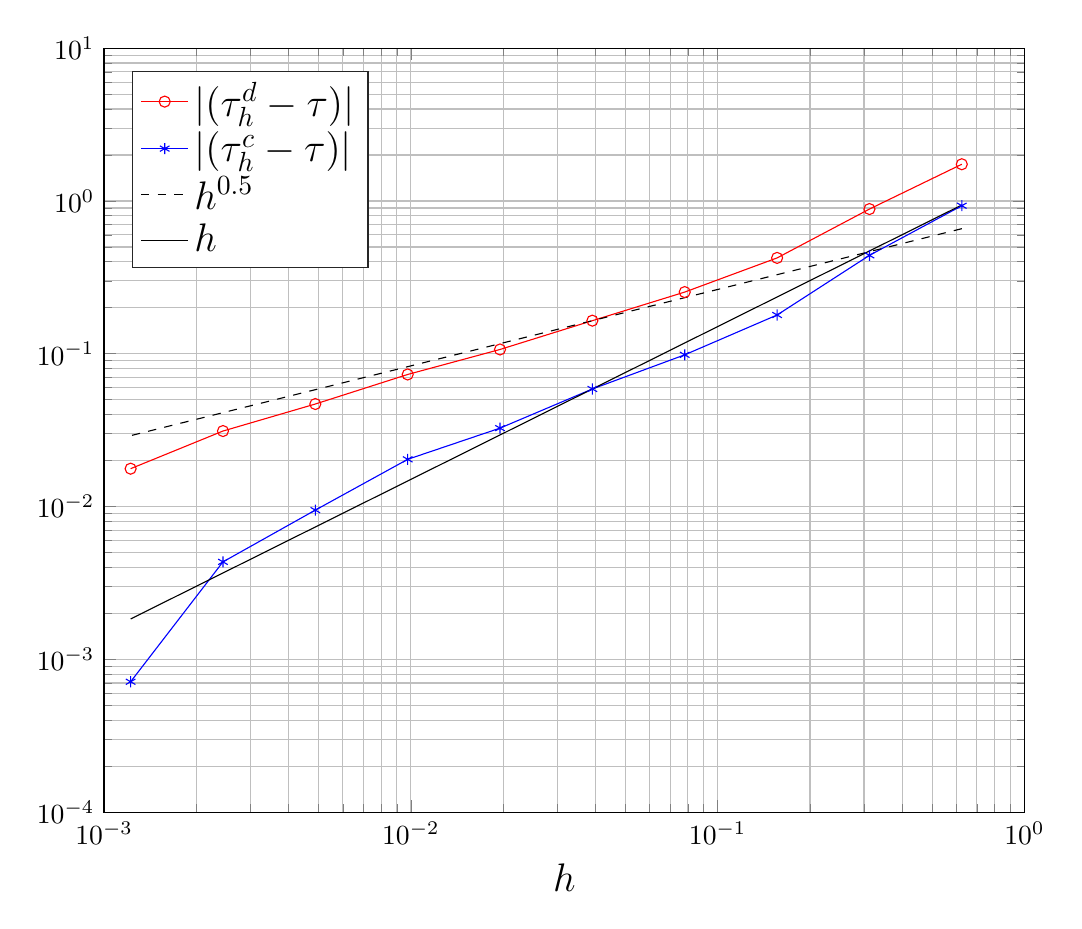
\begin{tikzpicture}

\begin{axis}[%
width=4.602in,
height=3.82in,
at={(0.772in,0.516in)},
scale only axis,
xmode=log,
xmin=0.001,
xmax=1,
xminorticks=true,
xlabel={$h$},
xlabel style={font=\Large},
xmajorgrids,
xminorgrids,
ymode=log,
ymin=0.0001,
ymax=10,
yminorticks=true,
ymajorgrids,
yminorgrids,
axis background/.style={fill=white},
legend style={at={(0.03,0.97)},anchor=north west,legend cell align=left,align=left,draw=white!15!black,font=\Large}
]
\addplot [color=red,solid,mark=o,mark options={solid}]
  table[row sep=crcr]{%
0.625	1.73914617431998\\
0.3125	0.885146174319978\\
0.15625	0.423927424319978\\
0.078125	0.253357111819978\\
0.0390625	0.164665705569978\\
0.01953125	0.106693049319978\\
0.009765625	0.0732106274449781\\
0.0048828125	0.0468932446324781\\
0.00244140625	0.0312094067418531\\
0.001220703125	0.0176961010777906\\
};
\addlegendentry{$|\E(\tau_h^d - \tau)|$};

\addplot [color=blue,solid,mark=asterisk,mark options={solid}]
  table[row sep=crcr]{%
0.625	0.931021174319978\\
0.3125	0.440614924319978\\
0.15625	0.179380549319978\\
0.078125	0.098419611819978\\
0.0390625	0.058821955569978\\
0.01953125	0.0326110180699781\\
0.009765625	0.0203737133824781\\
0.0048828125	0.00948064697622808\\
0.00244140625	0.00434612549185309\\
0.001220703125	0.000713688961271941\\
};
\addlegendentry{$|\E(\tau_h^c - \tau)|$};

\addplot [color=black,dashed]
  table[row sep=crcr]{%
0.625	0.658662822279912\\
0.3125	0.465744948149596\\
0.15625	0.329331411139956\\
0.078125	0.232872474074798\\
0.0390625	0.164665705569978\\
0.01953125	0.116436237037399\\
0.009765625	0.082332852784989\\
0.0048828125	0.0582181185186995\\
0.00244140625	0.0411664263924945\\
0.001220703125	0.0291090592593497\\
};
\addlegendentry{$h^{0.5}$};

\addplot [color=black,solid]
  table[row sep=crcr]{%
0.625	0.941151289119649\\
0.3125	0.470575644559824\\
0.15625	0.235287822279912\\
0.078125	0.117643911139956\\
0.0390625	0.058821955569978\\
0.01953125	0.029410977784989\\
0.009765625	0.0147054888924945\\
0.0048828125	0.00735274444624726\\
0.00244140625	0.00367637222312363\\
0.001220703125	0.00183818611156181\\
};
\addlegendentry{$h$};

\end{axis}
\end{tikzpicture}%
 }  
        \caption{Reflecting boundary in $x = 1$}
        \label{fig:ReflectOneD}
    \end{subfigure}    
    \caption{Approximation of $\tau$. Orders of convergence for DEM and CEM in the one-dimensional case.}
    \label{fig:OrdersOneD}
\end{figure}

\begin{figure}[t]
    \centering
    \begin{subfigure}{0.49\linewidth}
        \centering
        \resizebox{1\linewidth}{!}{% This file was created by matlab2tikz.
%
%The latest updates can be retrieved from
%  http://www.mathworks.com/matlabcentral/fileexchange/22022-matlab2tikz-matlab2tikz
%where you can also make suggestions and rate matlab2tikz.
%
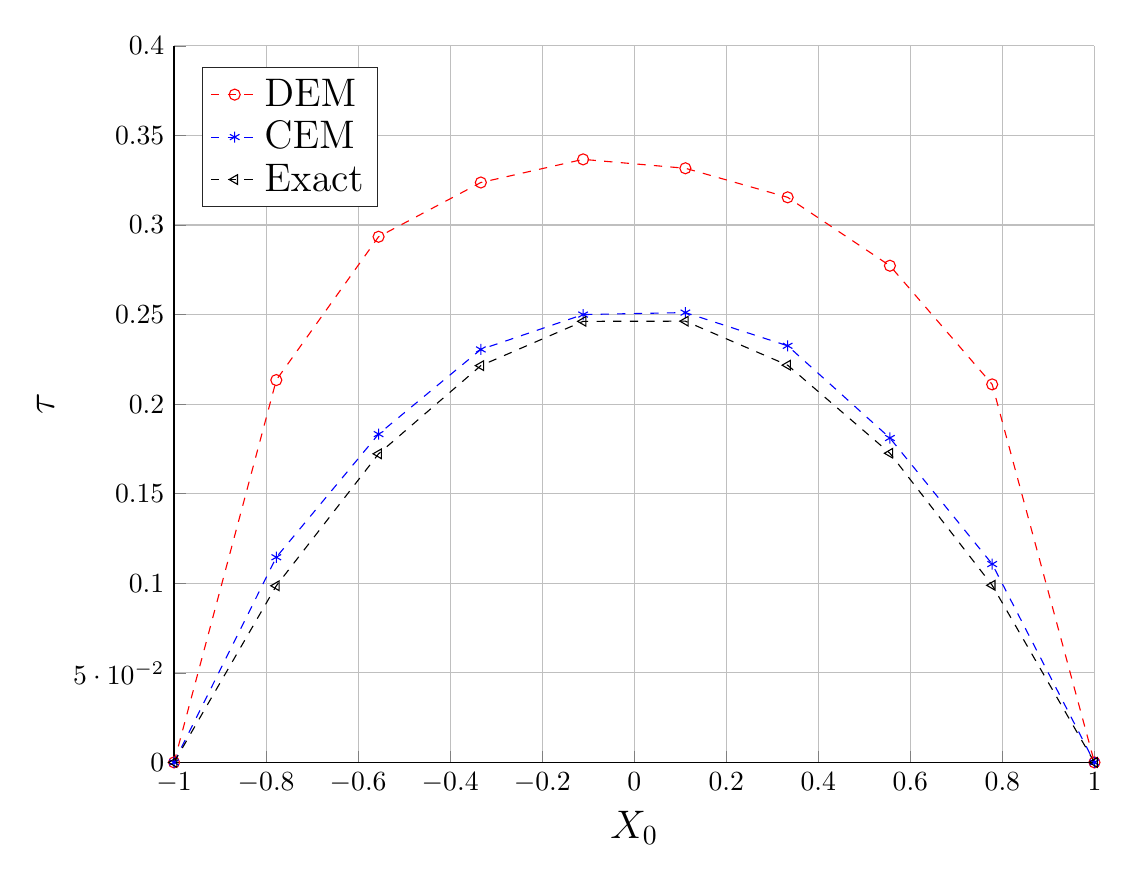
\begin{tikzpicture}

\begin{axis}[%
width=4.602in,
height=3.583in,
at={(0.772in,0.484in)},
scale only axis,
xmin=-1,
xmax=1,
xlabel={$X_0$},
xlabel style = {font = \Large},
xmajorgrids,
ymin=0,
ymax=0.4,
ylabel={$\tau$},
ylabel style = {font = \Large},
ymajorgrids,
axis background/.style={fill=white},
axis x line*=bottom,
axis y line*=left,
legend pos = north west,
legend style={legend cell align=left,align=left,draw=white!15!black,font=\Large}
]
\addplot [color=red,dashed,mark=o,mark options={solid}]
  table[row sep=crcr]{%
-1	0\\
-0.777777777777778	0.213421875\\
-0.555555555555556	0.2934140625\\
-0.333333333333333	0.3236953125\\
-0.111111111111111	0.336609375\\
0.111111111111111	0.331640625\\
0.333333333333333	0.315421875\\
0.555555555555556	0.2772421875\\
0.777777777777778	0.2110078125\\
1	0\\
};
\addlegendentry{DEM};

\addplot [color=blue,dashed,mark=asterisk,mark options={solid}]
  table[row sep=crcr]{%
-1	0\\
-0.777777777777778	0.114515625\\
-0.555555555555556	0.1832578125\\
-0.333333333333333	0.2305078125\\
-0.111111111111111	0.249984375\\
0.111111111111111	0.2510859375\\
0.333333333333333	0.232546875\\
0.555555555555556	0.181078125\\
0.777777777777778	0.11071875\\
1	0\\
};
\addlegendentry{CEM};

\addplot [color=black,dashed,mark=triangle,mark options={solid,rotate=90}]
  table[row sep=crcr]{%
-1	0\\
-0.777777777777778	0.0986011931395157\\
-0.555555555555556	0.172254291984329\\
-0.333333333333333	0.221472162307402\\
-0.111111111111111	0.246204174763737\\
0.111111111111111	0.2462957329545\\
0.333333333333333	0.221719125026098\\
0.555555555555556	0.172574095814315\\
0.777777777777778	0.0988572350577004\\
1	0\\
};
\addlegendentry{Exact};

\end{axis}
\end{tikzpicture}%
 }  
        \caption{Killing boundary in $x = 1$}
        \label{fig:ApproxOneD}
    \end{subfigure}
    \begin{subfigure}{0.49\linewidth}
        \centering
        \resizebox{1\linewidth}{!}{% This file was created by matlab2tikz.
%
%The latest updates can be retrieved from
%  http://www.mathworks.com/matlabcentral/fileexchange/22022-matlab2tikz-matlab2tikz
%where you can also make suggestions and rate matlab2tikz.
%
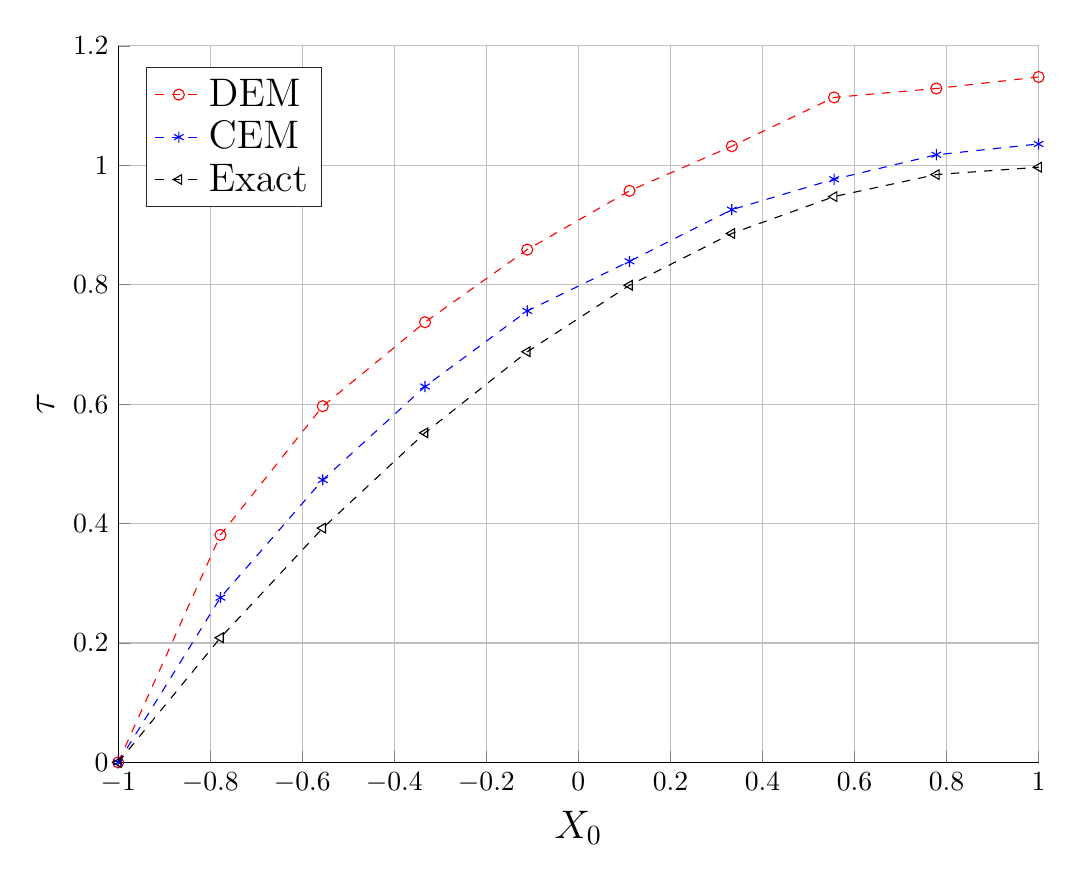
\begin{tikzpicture}

\begin{axis}[%
width=4.602in,
height=3.583in,
at={(0.772in,0.484in)},
scale only axis,
xmin=-1,
xmax=1,
xlabel={$X_0$},
xlabel style={font=\Large},
xmajorgrids,
ymin=0,
ymax=1.2,
ylabel={$\tau$},
ylabel style={font=\Large},
ymajorgrids,
axis background/.style={fill=white},
axis x line*=bottom,
axis y line*=left,
legend pos = north west,
legend style={legend cell align=left,align=left,draw=white!15!black,font=\Large}
]
\addplot [color=red,dashed,mark=o,mark options={solid}]
  table[row sep=crcr]{%
-1	0\\
-0.777777777777778	0.3809765625\\
-0.555555555555556	0.5964609375\\
-0.333333333333333	0.73715625\\
-0.111111111111111	0.8587265625\\
0.111111111111111	0.9571171875\\
0.333333333333333	1.031859375\\
0.555555555555556	1.113609375\\
0.777777777777778	1.1285390625\\
1	1.1478046875\\
};
\addlegendentry{DEM};

\addplot [color=blue,dashed,mark=asterisk,mark options={solid}]
  table[row sep=crcr]{%
-1	0\\
-0.777777777777778	0.275953125\\
-0.555555555555556	0.4729921875\\
-0.333333333333333	0.629484375\\
-0.111111111111111	0.7560703125\\
0.111111111111111	0.8390625\\
0.333333333333333	0.9255703125\\
0.555555555555556	0.976546875\\
0.777777777777778	1.017515625\\
1	1.035609375\\
};
\addlegendentry{CEM};

\addplot [color=black,dashed,mark=triangle,mark options={solid,rotate=90}]
  table[row sep=crcr]{%
-1	0\\
-0.777777777777778	0.208777054487475\\
-0.555555555555556	0.392333503315235\\
-0.333333333333333	0.551939853868488\\
-0.111111111111111	0.687661056545228\\
0.111111111111111	0.79906851214989\\
0.333333333333333	0.885727939207175\\
0.555555555555556	0.947463001823471\\
0.777777777777778	0.984384604394486\\
1	0.996687130893952\\
};
\addlegendentry{Exact};

\end{axis}
\end{tikzpicture}%
 }  
        \caption{Reflecting boundary in $x = 1$}
        \label{fig:ApproxOneD}
    \end{subfigure}    
    \caption{Approximation of $\tau$ as a function of the initial value $X_0$.}
    \label{fig:ApproxOneD}
\end{figure}


% Rough case is not useful anymore
\iffalse
\vspace{2mm}
\noindent\textbf{Rough case.} We consider the same domain $D$ as above, $T = 5$ and $g = \sigma = 3$. We consider $V$ to be piecewise linear, so that $f = -dV$ is piecewise constant. In particular, we choose the following form for $V$
\begin{equation}\label{eq:FunctionsOneDRough}
V = 0.1 
\left \{
\begin{aligned}
	 -2x -1&, && x < -0.5, \\
	 4x + 2&, && -0.5 \leq x < 0, \\
	 -2x + 2&, &&  0 \leq x < 0.5, \\
	 4x - 1&, && x \geq 0.5.
\end{aligned} \right .
\end{equation}
This is a linear interpolation of the function $V$ we used in the smooth case above in the points $\{-1,-0.5,0,0.5,1\}$. This case is of particular interest, since if the function $f$ is the result of a numerical method on a $PDE$, it could not be smooth as in the previous case. We perform DEM and CEM with the same parameters as before, \textit{i.e.}, $M = 10^4, N = 2^i,i=3,\dots,12$. In Figure \ref{fig:OrdersOneDRough} it is possible to remark that the rate of convergence of DEM is unvaried with respect to the previous case. The CEM method experiences a slight decrease in the order of convergence with respect to the smooth case.


\begin{figure}[t]
    \centering
    \begin{subfigure}{0.49\linewidth}
        \centering
        \resizebox{1\linewidth}{!}{\input{OneDCase/OrderKillRough.tikz} }  
        \caption{Killing boundary in $x = 1$}
        \label{fig:KillOneDRough}
    \end{subfigure}
    \begin{subfigure}{0.49\linewidth}
        \centering
        \resizebox{1\linewidth}{!}{\input{OneDCase/OrderReflRough.tikz} }  
        \caption{Reflecting boundary in $x = 1$}
        \label{fig:ReflectOneDRough}
    \end{subfigure}    
    \caption{Approximation of $\tau$. Orders of convergence for DEM and CEM in the one-dimensional case with $f$ piecewise constant.}
    \label{fig:OrdersOneDRough}
\end{figure}

\fi


\vspace{2mm}
\noindent \textbf{Estimation of the exit probability.} We consider \eqref{eq:OneDModel} with $D = \left[ -1, 1 \right]$, the final time $T = 1$, initial condition $X_0 = 0$ and we define
\begin{align}\label{eq:FunctionsOneDSmoothPhi}
\begin{split}
	f(x) &= -V'(x), \text{ where } V(x) = 0.1(8x^4 - 8x^2 + x + 2), \\
	g(x) &= \sigma = 2.
\end{split}
\end{align}
In order to approximate $\Phi$, we perform a Montecarlo simulation using both DEM and CEM, with $M = 10^5$ trajectories. We consider the number of timesteps for the time integration to be $N = 2^i, i = 3, \dots, 9$. The reference solution used to compute errors is obtained with Finite Differences applied to problem \eqref{eq:PDEPhi} (see Appendix \ref{sec:Appendix2}). Numerical results (Figure \ref{fig:KillOneDPhi}) confirm that the weak error for DEM is of order 0.5. For CEM it is not trivial to show a clear order of convergence one. This is due to the fact that the results are accurate already with a big step size, therefore the statistical error is not negligible with respect to the error due to time integration. In order to avoid the noise on the order of convergence, it would be necessary to increase the number of trajectories dramatically, leading to unaffordable computational times. Let us remark that CEM approximates the exit probability better than DEM for any initial value $X_0$, as shown in Figure \ref{fig:PhiProfiles}.

\begin{figure}[t]
    \centering
    \begin{subfigure}{0.49\linewidth}
        \centering
        \resizebox{1\linewidth}{!}{% This file was created by matlab2tikz.
%
%The latest updates can be retrieved from
%  http://www.mathworks.com/matlabcentral/fileexchange/22022-matlab2tikz-matlab2tikz
%where you can also make suggestions and rate matlab2tikz.
%
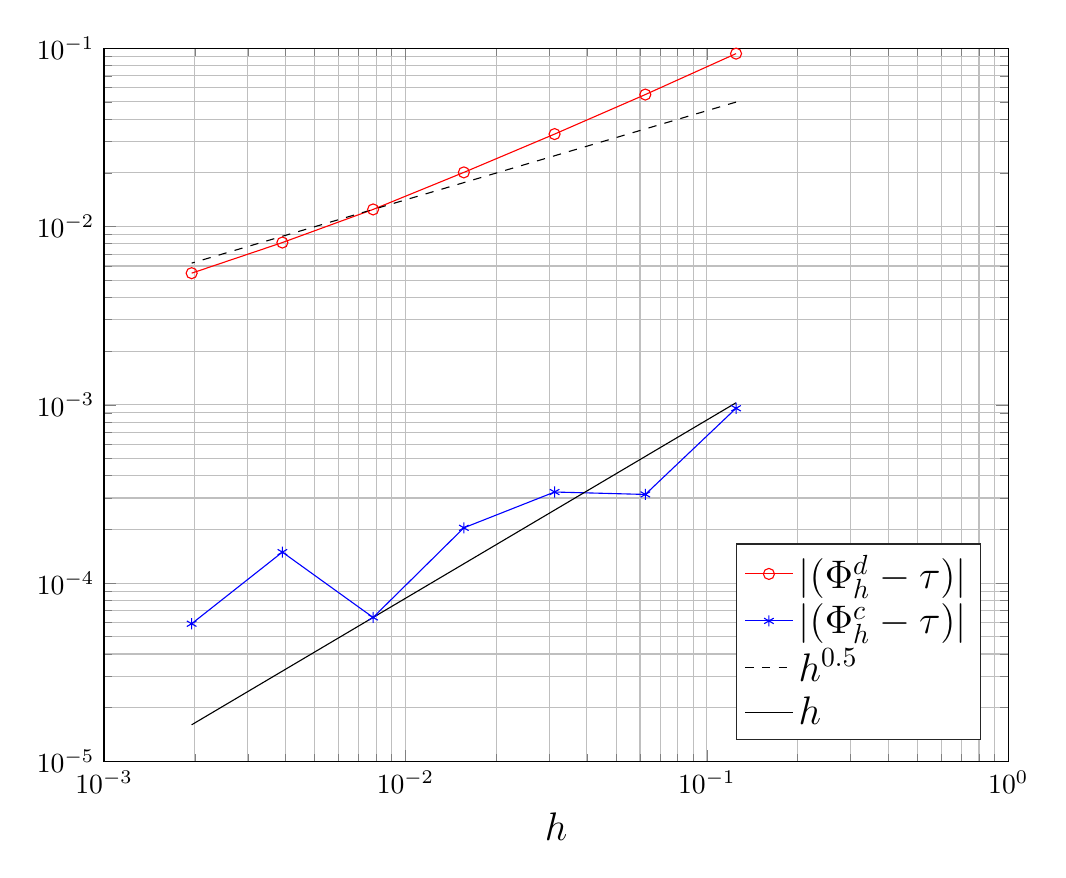
\begin{tikzpicture}

\begin{axis}[%
width=4.521in,
height=3.566in,
at={(0.758in,0.481in)},
scale only axis,
xmode=log,
xmin=0.001,
xmax=1,
xminorticks=true,
xlabel={$h$},
xlabel style={font=\Large},
xmajorgrids,
xminorgrids,
ymode=log,
ymin=1e-05,
ymax=0.1,
yminorticks=true,
ymajorgrids,
yminorgrids,
axis background/.style={fill=white},
legend pos = south east,
legend style={legend cell align=left,align=left,draw=white!15!black,font=\Large}
]
\addplot [color=red,solid,mark=o,mark options={solid}]
  table[row sep=crcr]{%
0.125	0.0931958331986392\\
0.0625	0.0549308331986392\\
0.03125	0.0329758331986393\\
0.015625	0.0201058331986392\\
0.0078125	0.0124608331986392\\
0.00390625	0.00812583319863924\\
0.001953125	0.00547083319863928\\
};
\addlegendentry{$|\E(\Phi_h^d - \tau)|$};

\addplot [color=blue,solid,mark=asterisk,mark options={solid}]
  table[row sep=crcr]{%
0.125	0.000955833198639233\\
0.0625	0.00031416680136076\\
0.03125	0.000324166801360715\\
0.015625	0.000204166801360706\\
0.0078125	6.41668013607877e-05\\
0.00390625	0.000149166801360789\\
0.001953125	5.91668013607549e-05\\
};
\addlegendentry{$|\E(\Phi_h^c - \tau)|$};

\addplot [color=black,dashed]
  table[row sep=crcr]{%
0.125	0.0498433327945569\\
0.0625	0.035244558615969\\
0.03125	0.0249216663972784\\
0.015625	0.0176222793079845\\
0.0078125	0.0124608331986392\\
0.00390625	0.00881113965399225\\
0.001953125	0.00623041659931961\\
};
\addlegendentry{$h^{0.5}$};

\addplot [color=black,solid]
  table[row sep=crcr]{%
0.125	0.0010266688217726\\
0.0625	0.000513334410886301\\
0.03125	0.000256667205443151\\
0.015625	0.000128333602721575\\
0.0078125	6.41668013607877e-05\\
0.00390625	3.20834006803938e-05\\
0.001953125	1.60417003401969e-05\\
};
\addlegendentry{$h$};

\end{axis}
\end{tikzpicture}%
 }  
        \caption{Killing boundary in $x = 1$}
        \label{fig:KillOneDPhi}
    \end{subfigure}
    \begin{subfigure}{0.49\linewidth}
        \centering
        \resizebox{1\linewidth}{!}{% This file was created by matlab2tikz.
%
%The latest updates can be retrieved from
%  http://www.mathworks.com/matlabcentral/fileexchange/22022-matlab2tikz-matlab2tikz
%where you can also make suggestions and rate matlab2tikz.
%
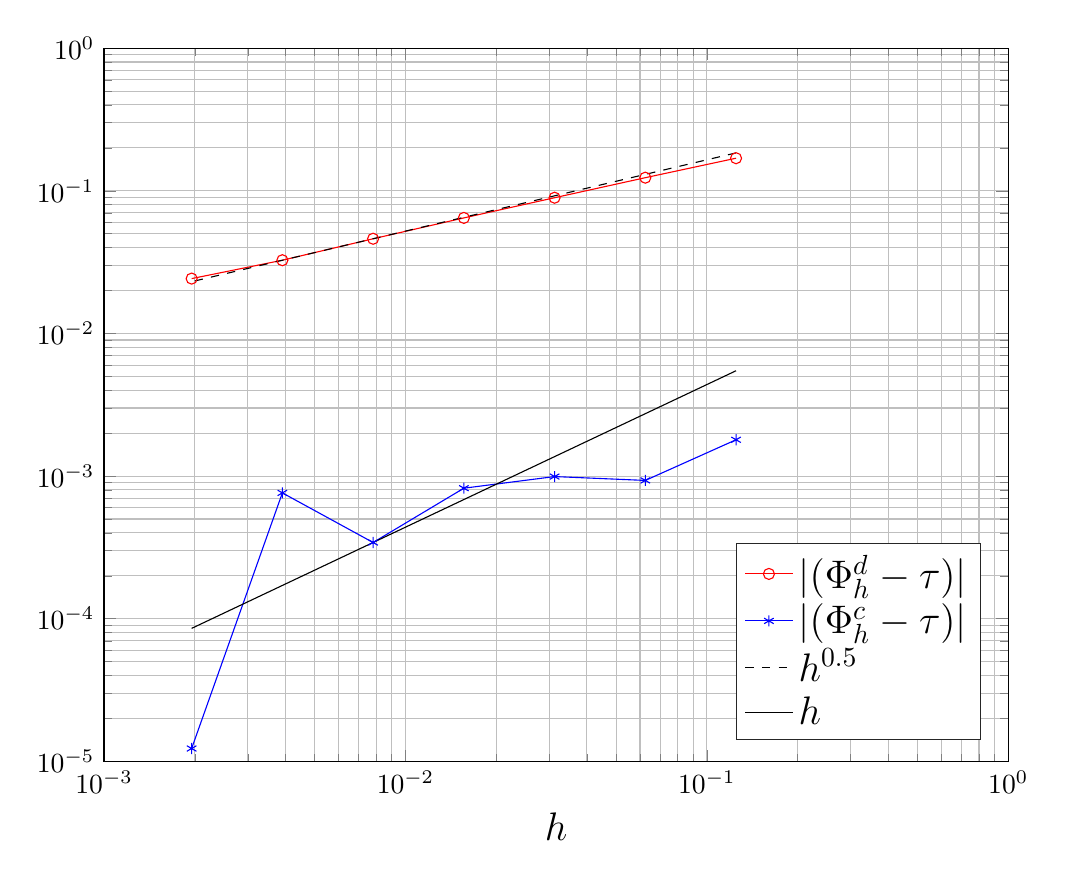
\begin{tikzpicture}

\begin{axis}[%
width=4.521in,
height=3.566in,
at={(0.758in,0.481in)},
scale only axis,
xmode=log,
xmin=0.001,
xmax=1,
xminorticks=true,
xlabel={$h$},
xlabel style = {font=\Large},
xmajorgrids,
xminorgrids,
ymode=log,
ymin=1e-05,
ymax=1,
yminorticks=true,
ymajorgrids,
yminorgrids,
axis background/.style={fill=white},
legend pos = south east,
legend style={legend cell align=left,align=left,draw=white!15!black,font=\Large}
]
\addplot [color=red,solid,mark=o,mark options={solid}]
  table[row sep=crcr]{%
0.125	0.169237691826179\\
0.0625	0.123577691826179\\
0.03125	0.0894376918261789\\
0.015625	0.0645576918261789\\
0.0078125	0.0461076918261789\\
0.00390625	0.032607691826179\\
0.001953125	0.024237691826179\\
};
\addlegendentry{$|\E(\Phi_h^d - \tau)|$};

\addplot [color=blue,solid,mark=asterisk,mark options={solid}]
  table[row sep=crcr]{%
0.125	0.00179769182617895\\
0.0625	0.000932308173821061\\
0.03125	0.000992308173821121\\
0.015625	0.000822308173821118\\
0.0078125	0.000342308173821082\\
0.00390625	0.000762308173821058\\
0.001953125	1.23081738211406e-05\\
};
\addlegendentry{$|\E(\Phi_h^c - \tau)|$};

\addplot [color=black,dashed]
  table[row sep=crcr]{%
0.125	0.184430767304716\\
0.0625	0.130412246220603\\
0.03125	0.0922153836523578\\
0.015625	0.0652061231103013\\
0.0078125	0.0461076918261789\\
0.00390625	0.0326030615551507\\
0.001953125	0.0230538459130895\\
};
\addlegendentry{$h^{0.5}$};

\addplot [color=black,solid]
  table[row sep=crcr]{%
0.125	0.00547693078113731\\
0.0625	0.00273846539056866\\
0.03125	0.00136923269528433\\
0.015625	0.000684616347642164\\
0.0078125	0.000342308173821082\\
0.00390625	0.000171154086910541\\
0.001953125	8.55770434552705e-05\\
};
\addlegendentry{$h$};

\end{axis}
\end{tikzpicture}%
 }  
        \caption{Reflecting boundary in $x = 1$}
        \label{fig:ReflectOneDPhi}
    \end{subfigure}    
    \caption{Approximation of $\Phi$. Orders of convergence of DEM and CEM in the one-dimensional case.}
    \label{fig:OrdersOneDPhi}
\end{figure}

\begin{figure}[t]
    \centering
    \begin{subfigure}{0.49\linewidth}
        \centering
        \resizebox{1\linewidth}{!}{% This file was created by matlab2tikz.
%
%The latest updates can be retrieved from
%  http://www.mathworks.com/matlabcentral/fileexchange/22022-matlab2tikz-matlab2tikz
%where you can also make suggestions and rate matlab2tikz.
%
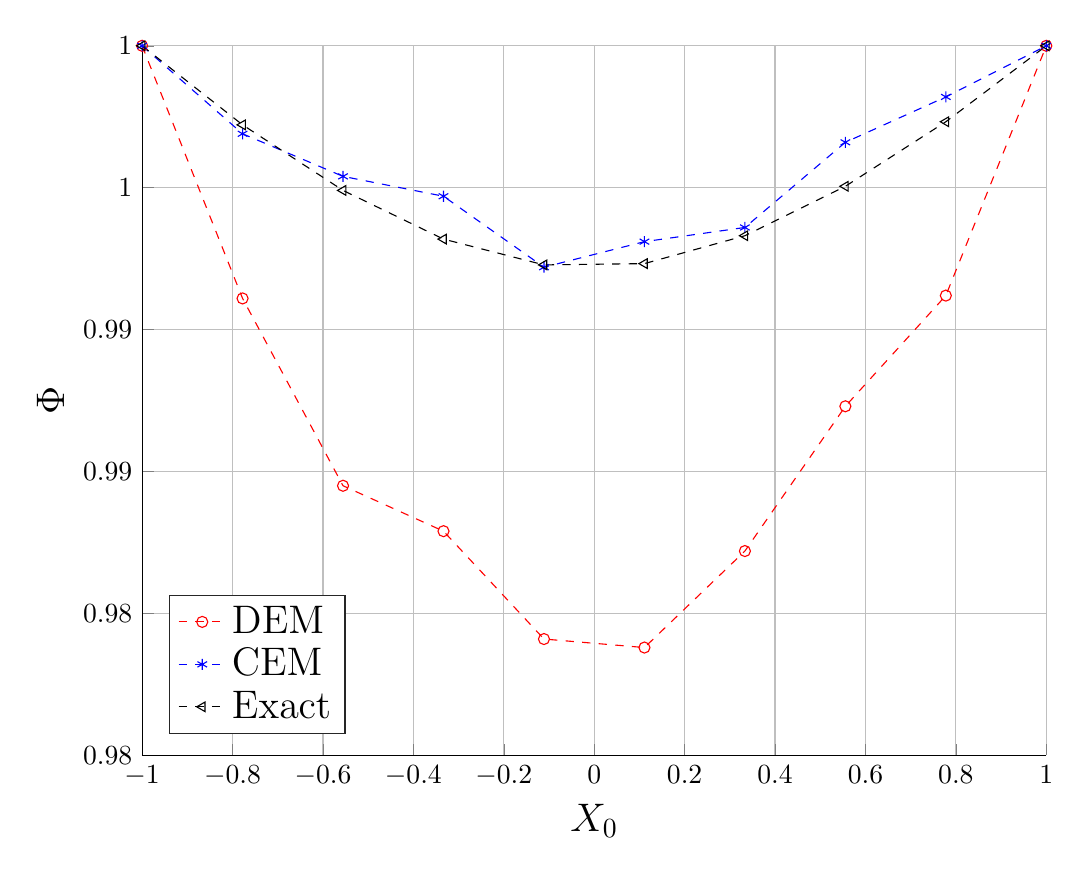
\begin{tikzpicture}

\begin{axis}[%
width=4.521in,
height=3.548in,
at={(0.758in,0.499in)},
scale only axis,
xmin=-1,
xmax=1,
xlabel={$X_0$},
xlabel style={font=\Large},
xmajorgrids,
ymin=0.975,
ymax=1,
ylabel={$\Phi$},
ylabel style={font=\Large},
ymajorgrids,
axis background/.style={fill=white},
axis x line*=bottom,
axis y line*=left,
legend style={at={(0.03,0.03)},anchor=south west,legend cell align=left,align=left,draw=white!15!black,font=\Large}
]
\addplot [color=red,dashed,mark=o,mark options={solid}]
  table[row sep=crcr]{%
-1	1\\
-0.777777777777778	0.9911\\
-0.555555555555556	0.9845\\
-0.333333333333333	0.9829\\
-0.111111111111111	0.9791\\
0.111111111111111	0.9788\\
0.333333333333333	0.9822\\
0.555555555555556	0.9873\\
0.777777777777778	0.9912\\
1	1\\
};
\addlegendentry{DEM};

\addplot [color=blue,dashed,mark=asterisk,mark options={solid}]
  table[row sep=crcr]{%
-1	1\\
-0.777777777777778	0.9969\\
-0.555555555555556	0.9954\\
-0.333333333333333	0.9947\\
-0.111111111111111	0.9922\\
0.111111111111111	0.9931\\
0.333333333333333	0.9936\\
0.555555555555556	0.9966\\
0.777777777777778	0.9982\\
1	1\\
};
\addlegendentry{CEM};

\addplot [color=black,dashed,mark=triangle,mark options={solid,rotate=90}]
  table[row sep=crcr]{%
-1	1\\
-0.777777777777778	0.99721538712255\\
-0.555555555555556	0.9949049913465\\
-0.333333333333333	0.993189956945965\\
-0.111111111111111	0.992280836629584\\
0.111111111111111	0.992326354174843\\
0.333333333333333	0.993308817442632\\
0.555555555555556	0.99505043807726\\
0.777777777777778	0.997324464142556\\
1	1\\
};
\addlegendentry{Exact};

\end{axis}
\end{tikzpicture}%
 }  
        \caption{Killing boundary in $x = 1$}
        \label{fig:KillPhiProfiles}
    \end{subfigure}
    \begin{subfigure}{0.49\linewidth}
        \centering
        \resizebox{1\linewidth}{!}{% This file was created by matlab2tikz.
%
%The latest updates can be retrieved from
%  http://www.mathworks.com/matlabcentral/fileexchange/22022-matlab2tikz-matlab2tikz
%where you can also make suggestions and rate matlab2tikz.
%
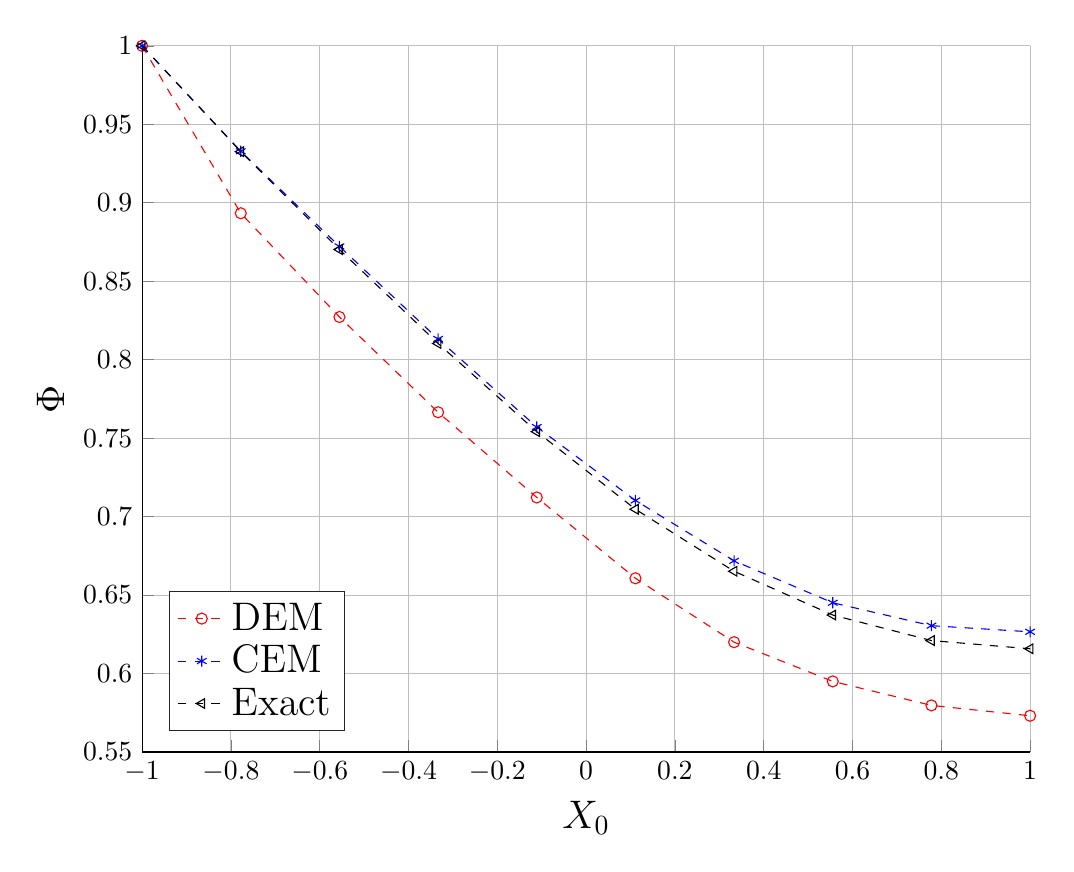
\begin{tikzpicture}

\begin{axis}[%
width=4.44in,
height=3.531in,
at={(0.745in,0.496in)},
scale only axis,
xmin=-1,
xmax=1,
xlabel={$X_0$},
xlabel style={font=\Large},
xmajorgrids,
ymin=0.55,
ymax=1,
ylabel={$\Phi$},
ylabel style={font=\Large},
ymajorgrids,
axis background/.style={fill=white},
axis x line*=bottom,
axis y line*=left,
legend style={at={(0.03,0.03)},anchor=south west,legend cell align=left,align=left,draw=white!15!black,font = \Large}
]
\addplot [color=red,dashed,mark=o,mark options={solid}]
  table[row sep=crcr]{%
-1	1\\
-0.777777777777778	0.8933\\
-0.555555555555556	0.8272\\
-0.333333333333333	0.7665\\
-0.111111111111111	0.7122\\
0.111111111111111	0.6607\\
0.333333333333333	0.62\\
0.555555555555556	0.595\\
0.777777777777778	0.5797\\
1	0.5731\\
};
\addlegendentry{DEM};

\addplot [color=blue,dashed,mark=asterisk,mark options={solid}]
  table[row sep=crcr]{%
-1	1\\
-0.777777777777778	0.9328\\
-0.555555555555556	0.8722\\
-0.333333333333333	0.8132\\
-0.111111111111111	0.7571\\
0.111111111111111	0.7103\\
0.333333333333333	0.6718\\
0.555555555555556	0.6451\\
0.777777777777778	0.6305\\
1	0.6266\\
};
\addlegendentry{CEM};

\addplot [color=black,dashed,mark=triangle,mark options={solid,rotate=90}]
  table[row sep=crcr]{%
-1	1\\
-0.777777777777778	0.932548077502788\\
-0.555555555555556	0.870181977112059\\
-0.333333333333333	0.810303153980793\\
-0.111111111111111	0.754108688988762\\
0.111111111111111	0.70469446885863\\
0.333333333333333	0.665180416423286\\
0.555555555555556	0.63727357440893\\
0.777777777777778	0.621019342130665\\
1	0.615785886384429\\
};
\addlegendentry{Exact};

\end{axis}
\end{tikzpicture}%
 }  
        \caption{Reflecting boundary in $x = 1$}
        \label{fig:ReflectPhiProfiles}
    \end{subfigure}    
    \caption{Approximation of $\Phi$ as a function of the initial value $X_0$.}
    \label{fig:PhiProfiles}
\end{figure}




